\documentclass[paper]{aiaaNew}

\usepackage{amssymb}
\usepackage{bm}
\usepackage{amsthm}% http://ctan.org/pkg/amsthm
\usepackage{amsmath}
\usepackage[linewidth=1pt]{mdframed}
\usepackage{graphicx}
\usepackage{algorithm}
\usepackage{algpseudocode}
\usepackage{longtable,tabularx}
\newcommand{\norm}[1]{\left\lVert#1\right\rVert}
% \documentclass[conf]{new-aiaa}
\usepackage[utf8]{inputenc}

% \usepackage[utf8]{inputenc}
% \usepackage{subcaption}
% \usepackage{sidecap}
% \usepackage{mathtools}
% \usepackage{commath}
% \usepackage{listings}
% \usepackage[version=4]{mhchem}
% \usepackage{siunitx}
% \usepackage{amsmath,amsfonts,bm} % Math packages
% \setlength\LTleft{0pt} 


% \usepackage{longtable,tabularx}
% \usepackage[utf8]{inputenc}


% \newenvironment{proof}
% {}{}


%\documentstyle[10pt,draft,fancyheadings]{AIAAtran}
%\documentstyle[9pt,twocolumn,technote,twoside]{AIAAtran}


\SubmitName{Lysandrou}
% for conference paper:
\PaperNumber{xxx}
\CoverFigure{}
\Conference{{\bfseries AIAA Guidance, Navigation and \\ Control 
Conference} \\
            August 10--12,~1998 / Boston, MA}

% for a journal simulation cover page:
\JournalName{Journal of Guidance, Navigation and Control}
\JournalIssue{Volume~xx, Number~xx, Jan.--Feb., 2001, Pages xx--xx}
% journal article simulation:
\ArticleIssue{Vol.~24, No.~1, Jan.--Feb., 2001}% first page
\ArticleHeader{Schaub Et Al: New Penalty Functions}% subsequent pages
% journal note simulation:
\NoteHeader{J.Guidance, Vol.~20, No.~13: Engineering Notes}
% set copyright and other notices to appear
% as a footnote at the bottom of the first page:
%\PaperNotice{\CopyrightB{1998}{Hanspeter Schaub}}
\JournalNotice{Presented as Paper~06--3792 at the AIAA
               Guidance, Navigation and Control Conference, San 
Diego,~CA,               July~29--31,~1996.
               \CopyrightB{1996}{the authors}}
% load the title, author, and abstract for use with the \maketitle command




\title{Attitude Dynamics and Control of a Nano-Satellite Orbiting Mars}
\author{Padraig S. Lysandrou
  \thanks{PhD Student, Aerospace Engineering Department.  Student Member of AIAA.}
  \\
  \emph{\normalsize The University of Colorado Boulder, Boulder, CO 80301}
}

\abstract{
This project for ASEN5010 Spacecraft Dynamics and Control considers a small satellite orbiting Mars at a low altitude. This spacecraft gathers science data and transfers this data to another satellite orbiting at a higher altitude. Periodically, this spacecraft must transition from nadir-pointing, science gathering mode to sun-pointing mode to recharge the battery system. The three missions goals are nadir-pointing, communicating with the mother spacecraft, and to sun-point. Both of these spacecraft are in circular orbits.}

\begin{document}
\maketitle


\clearpage
\section{Introduction}

\section{Problem Statement}
Let us begin with defining the orbit of the nano-satellite with the following figure


\begin{figure}[!htbp] 
  \centering
  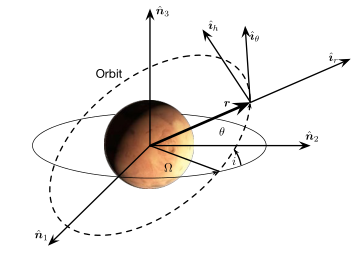
\includegraphics[width=0.5\textwidth]{Figures/framedef.PNG}
  \caption{Illustration of the Inertial, Hill, and perifocal geometrical constructions. Taken from ASEN5010 Semester Project sheet.}
  \label{fig:succ}
 \end{figure}



\section*{Task 1: Orbit Simulation}
Our Hill frame is defined by the basis: $\{\bm{\hat{i}}_r, \bm{\hat{i}}_\theta, \bm{\hat{i}}_h \}$ with the inertial defined as $\{\bm{\hat{n}}_1, \bm{\hat{n}}_2, \bm{\hat{n}}_3 \}$. Given the inertial and Hill frame definitions, we know that the position vector of the LMO satellite is $r\bm{\hat{i}}_r$. Additionally we know that since it is a circular orbit, it has a time invariant angular rate ${\bm{\omega}}_{H/N} = \dot{\theta}\mathbf{\hat{i}}_h$. Calculating the vectorial inertial derivative:

\begin{align}
	\dot{\bm{r}} = \frac{^N d}{dt}\bm{r} &= \frac{^H d}{dt}\bm{r} + \bm{\omega}_{H/N} \times \bm{r} \\
	&= \dot{\theta}\bm{\hat{i}}_h \times r\bm{\hat{i}}_r \\
	&= r\dot{\theta} \bm{\hat{i}}_\theta
\end{align}

Additionally, we can use this information to find the inertial position and velocity vectors by performing transformations using the perifocal frame information. We know that the perifocal frame can be defined by an Euler 3-1-3 rotation defined the set $\{\Omega, i, \theta \}$

\begin{equation}
C_{ECI} = 
\begin{bmatrix}
\cos{\theta} & \sin{\theta} & 0 \\
-\sin{\theta} & \cos{\theta} & 0 \\
0 & 0 & 1 
\end{bmatrix}
\begin{bmatrix}
1 & 0 & 0 \\
0 & \cos{i} & \sin{i} \\
0 & -\sin{i} & \cos{i} \\
\end{bmatrix}
\begin{bmatrix}
\cos{\Omega} & \sin{\Omega} & 0 \\
-\sin{\Omega} & \cos{\Omega} & 0 \\
0 & 0 & 1 
\end{bmatrix}
\end{equation}

Which describes a rotation from Earth Centered Inertial frame. Each portion of the DCM is a single-axis rotation. We can then use this to project scalar values in the Hill frame to inertial vectors with the following:

\begin{align}
  ^N\vec{\bm{r}} &= C_{ECI}^T 
  \begin{bmatrix}
  r \\ 0 \\ 0
  \end{bmatrix} \\
  ^N\vec{\bm{v}} &= C_{ECI}^T
  \begin{bmatrix}
  0 \\ r\dot{\theta} \\ 0
  \end{bmatrix}
\end{align}

When the ECI direction cosine matrix is calculated, $\theta$ must be propagated over time, as the true anomaly is the only perifocal parameter that is time variant. It is calculate as such: $\theta = \theta_0 + t*\dot{\theta}$.







\section*{Task 2: Orbit Frame Orientation}
It is simple to generate bases vectors for the Hill frame, under motion, using our new inertial vectors. As stated before, $\mathcal{H} = \{\bm{\hat{i}}_r, \bm{\hat{i}}_\theta, \bm{\hat{i}}_h \}$, which can be constructed with the following:

\begin{align}
  \hat{\bm{i}_r} &= \frac{\bm{r}_{LM}}{\norm{\bm{r}_{LM}}} \\
  \hat{\bm{i}_\theta} &= \hat{\bm{i}_h} \times \hat{\bm{i}_r} \\
  \hat{\bm{i}_h} &= \frac{\bm{r}_{LM} \times \dot{\bm{r}}_{LM}}{\norm{\bm{r}_{LM} \times \dot{\bm{r}}_{LM}}}
\end{align}

If we stack up these vectors into a matrix $[\hat{\bm{i}_r} \ \hat{\bm{i}_\theta} \ \hat{\bm{i}_h}]$, this defines the direction cosine matrix which takes vectors in the Hill frame to the inertial frame: $[NH]$. We can take the transpose to find the opposite: $[HN] = [\hat{\bm{i}_r} \ \hat{\bm{i}_\theta} \ \hat{\bm{i}_h}]^T$.









\section*{Task 3: Sun-Pointing Reference Frame Orientation}
The solar panel axis $\hat{\bm{b}}_3$ must be pointed at the sun, and a reference frame $\mathcal{R}_s$ must be generated such that $\hat{\bm{r}}_3$ points in the sun direction ($\hat{\bm{n}}_2$). Given that the solar reference frame is constant with respect to the inertial frame, the $^N\bm{\omega}_{R_s N} = \bm{0}$. And our DCM is easily constructed using our assumptions with the following: 
\begin{align}
  [R_sN] =  
  \begin{bmatrix}
  -1 & 0 & 0 \\
  0 & 0 & 1 \\
  0 & 1 & 0
  \end{bmatrix}
\end{align}








\section*{Task 4: Nadir-Pointing Reference Frame Orientation}
In order to point the payload platform axis $\hat{\bm{b}}_1$ towards Mars in the nadir direction, the reference frame $\mathcal{R}_n$ must be constructed such that $\hat{\bm{r}}_1$ points towards the planet. Additionally, we assume that $\hat{\bm{r}}_2$ is in the direction of the velocity $\hat{\bm{i}}_\theta$. Therefore we easily can construct a Hill-to-reference DCM which, using our now stated definitions, follows as such: 

\begin{align}
  [R_nH] =  
  \begin{bmatrix}
  -1 & 0 & 0 \\
  0 & 1 & 0 \\
  0 & 0 & -1
  \end{bmatrix}
\end{align}

This is the manifestation of a simple $\pi$ rotation about the second Hill axis, where the reference flips $\hat{\bm{i}}_r$ and $\hat{\bm{i}}_h$. We can then calculate $[HN]$ using our procedure from Task 2. We then generate $[R_nN]$ via the following:

\begin{equation}
  [R_nN] = [R_nH][HN]
\end{equation}

Similarly, given that we are on a circular orbit, and that our reference is an invariant transformation from the Hill frame, we can easily describe $^N \bm{\omega}_{R_nN}$. Given that the reference and Hill angular rates are similar, we know that $^H \bm{\omega}_{R_nN} = [0 \ 0 \ \dot{\theta}]^T$ and can supply the reference angular rate with the following


\begin{equation}
  ^N \bm{\omega}_{R_nN} = [HN]^T \ ^H \bm{\omega}_{R_nN} = [NH][0 \ 0 \ \dot{\theta}]^T
\end{equation}







\section*{Task 5: GMO-Pointing Reference Frame Orientation}
Now we must construct another reference frame $\mathcal{R}_c$ such that $-\hat{\bm{r}}_1 = $ points towards the GMO spacecraft. This is simply done by finding the vector which represents the inertial difference in the position of both spacecraft: $\Delta\bm{r} = \bm{r}_{LMO} - \bm{r}_{GMO}$. We can then describe the frame with the following:

\begin{align}
  \hat{\bm{r}}_1 &= \frac{-\Delta\bm{r}}{\norm{\Delta\bm{r}}} \\ 
  \hat{\bm{r}}_2 &= \frac{\Delta\bm{r} \times \hat{\bm{n}}_3}{\norm{\Delta\bm{r} \times \hat{\bm{n}}_3}} \\ 
  \hat{\bm{r}}_3 &= \hat{\bm{r}}_1 \times \hat{\bm{r}}_2 
\end{align}

Stacking these unit vectors as such $[\hat{\bm{r}}_1 \ \hat{\bm{r}}_2 \ \hat{\bm{r}}_3 ]$ yields a rotation matrix that, when multiplied by, brings vectors from the tracking reference frame to the inertial frame. Therefore, under a transpose operation we get the following: 

\begin{equation}
  [R_cN] = [\hat{\bm{r}}_1 \ \hat{\bm{r}}_2 \ \hat{\bm{r}}_3 ]^T
\end{equation}

Finding $^N\bm{\omega}_{R_cN}$ is nontrivial and finding an analytical expression for the time derivative of the DCM can be challenging. Instead, we can use a numerical approach to find a usable solution. We know that the derivative of a DCM is that: $[\dot{C}] = -[\bm{\omega}^\times][C]$. Therefore we can find the angular rate with the following:



\begin{align}
  \frac{d[R_cN]}{dt} &= -[\bm{\omega_{R_cN}}^\times][R_cN] \\
  \frac{[R_cN(t+dt)] - [R_cN(t)]}{dt} [NR_c] &= -[\bm{\omega_{R_cN}}^\times]
\end{align}

Because we know have a function that determines this reference DCM at any point in time, this numerical derivative is easy to calculate for a small value $dt$. With knowledge of the skew symmetric form, we can de-skew $[\bm{\omega_{R_cN}}^\times]$ to find our vector  $^{R_c}\bm{\omega_{R_cN}}$. To bring this quantity into the inertial frame we perform $^{N}\bm{\omega_{R_cN}} = [R_cN(t)]^T \ ^{R_c}\bm{\omega_{R_cN}}$.






\section*{Task 6: Attitude and Angular Rate Error Evaluation}
In this section, we must write a function that, given a current attitude state $\bm{\sigma}_{BN}$, angular rate $^B\bm{\omega}_{BN}$, and desired reference attitude matrix $[RN]$, returns the associate tracking errors $\bm{\sigma}_{BR}$ and $^B\bm{\omega}_{BR}$. First let us start with the simpler angular velocity error:

\begin{equation}
  ^B\bm{\omega}_{BR} = (^B\bm{\omega}_{BN} - [BN] \ ^N\bm{\omega}_{RN})
\end{equation}

We can find the inertial to body DCM transform by performing $\text{MRP2C}(\bm{\sigma}_{BN})$ with the following function:

\begin{equation}
  [BN]=\frac{1}{\left(1+\sigma^{2}\right)^{2}}
  \begin{bmatrix}
    {4\left(\sigma_{1}^{2}-\sigma_{2}^{2}-\sigma_{3}^{2}\right)+\left(1-\sigma^{2}\right)^{2}} & {8 \sigma_{1} \sigma_{2}+4 \sigma_{3}\left(1-\sigma^{2}\right)} & {8 \sigma_{1} \sigma_{3}-4 \sigma_{2}\left(1-\sigma^{2}\right)} \\
    {8 \sigma_{2} \sigma_{1}-4 \sigma_{3}\left(1-\sigma^{2}\right)} & {4\left(-\sigma_{1}^{2}+\sigma_{2}^{2}-\sigma_{3}^{2}\right)+\left(1-\sigma^{2}\right)^{2}} & {8 \sigma_{2} \sigma_{3}+4 \sigma_{1}\left(1-\sigma^{2}\right)} \\
    {8 \sigma_{3} \sigma_{1}+4 \sigma_{2}\left(1-\sigma^{2}\right)} & {8 \sigma_{3} \sigma_{2}-4 \sigma_{1}\left(1-\sigma^{2}\right)} & {4\left(-\sigma_{1}^{2}-\sigma_{2}^{2}+\sigma_{3}^{2}\right)+\left(1-\sigma^{2}\right)^{2}} \\
  \end{bmatrix}
\end{equation}

Now that we have the tracking error for the angular velocity, we must find the relative error in the modified rodrigues parameter attitude formalism. We could use the relative MRP formula, but it can be understood more easily by converting to DCMs and using fundamental properties of the SO(3) group: 

\begin{equation}
  \bm{\sigma}_{BR} = \text{C2MRP}([BN][RN]^T)
\end{equation}

The DCM to MRP transform is more complicated and is done by first converting the DCM to a quaternion via Sheppard's method. The first step is to find the maximum of these values, as truth, to constrain that value for the second step:

\begin{equation}
  \begin{array}{ll}{\beta_{0}^{2}=\frac{1}{4}(1+\operatorname{tr}([BR]))} & {\beta_{2}^{2}=\frac{1}{4}\left(1+2 [BR]_{22}-\operatorname{tr}([BR])\right)} \\ {\beta_{1}^{2}=\frac{1}{4}\left(1+2 [BR]_{11}-\operatorname{tr}([BR])\right)} & {\beta_{3}^{2}=\frac{1}{4}\left(1+2 [BR]_{33}-\operatorname{tr}([BR])\right)}\end{array}
\end{equation}

The second step is done by computing the rest of the quaternion entries, using our constrained entry, with the following: 

\begin{equation}
  \begin{array}{ll}{\beta_{0} \beta_{1}=\left([BR]_{23}-[BR]_{32}\right) / 4} & {\beta_{1} \beta_{2}=\left([BR]_{12}+[BR]_{21}\right) / 4} \\ {\beta_{0} \beta_{2}=\left([BR]_{31}-[BR]_{13}\right) / 4} & {\beta_{3} \beta_{1}=\left([BR]_{31}+[BR]_{13}\right) / 4} \\ {\beta_{0} \beta_{3}=\left([BR]_{12}-[BR]_{21}\right) / 4} & {\beta_{2} \beta_{3}=\left([BR]_{23}+[BR]_{32}\right) / 4}\end{array}
\end{equation}

The final MRP is calculated with from our quaternion entries using the definition:

\begin{equation}
  \bm{\sigma}_{BR} = \begin{bmatrix}
  \frac{\beta_1}{1+\beta_0} \\
  \frac{\beta_2}{1+\beta_0} \\
  \frac{\beta_3}{1+\beta_0} 
  \end{bmatrix}
\end{equation}






\section*{Task 7: Numerical Attitude Simulator}
Now we must numerically integrate our differential equations of motion to simulate the dynamics of our system for both the LMO and GMO spacecraft. Let us define our state vector as the following: 

\begin{equation}
  \bm{X} = \begin{bmatrix}
  \bm{\sigma}_{BN} \\
  ^B\bm{\omega}_{BR}
  \end{bmatrix}
\end{equation}

For $\bm{u}$ control torque vector, the rigid body dynamics obey the following:

\begin{equation}
  [I]\bm{\dot{\omega}}_{BN} = -[\omega_{BN}^\times][I]\bm{\omega}_{BN} + \bm{u}
\end{equation}

We use a fourth order Runge-Kutte algorithm for integration (RK4). Using the nonlinear dynamics function $\dot{\bm{X}} = f(t,\bm{X})$, the integration algorithm is:



\begin{algorithm}
\caption{Fourth Order Runge Kutte Integrator}\label{RK4}
\begin{algorithmic}[1]
\For{i = 1:N-1} 
    \State $ k_1 = \dot{\bm{X}}(t(i), \ \bm{X}(:,i))$
    \State $ k_2 = \dot{\bm{X}}(t(i)+ \frac{dt}{2}, \  \bm{X}(:,i)+ \frac{dt}{2} k_1)$
    \State $ k_3 = \dot{\bm{X}}(t(i)+ \frac{dt}{2}, \ \bm{X}(:,i)+ \frac{dt}{2} k_2)$
    \State $ k_4 = \dot{\bm{X}}(t(i)+dt,  \ \bm{X}(:,i) + dt k_3)$
    \State $ \bm{X}(:,i+1) =  \bm{X}(:,i) + \frac{dt}{6}(k_1+2k_2+2k_3+k_4)$
\EndFor
\end{algorithmic}
\end{algorithm}

Each point $i \in [1:N]$ is 1 integration time step, and therefore the full simulation time $dtN$. Using this simulation framework, we can study our angular momentum $\bm{H} = [I]\bm{\omega}_{BN}$ and kinetic energy $T = \frac{1}{2} \bm{\omega}_{BN}^T [I] \bm{\omega}_{BN}$ over time.


% for i = 1:npoints-1






\section{Conclusion}

\section*{Acknowledgment}

\bibliographystyle{aiaa}   % Number the references.
\bibliography{references}   % Use references.bib to resolve the labels.


\end{document}

